\begin{frame}{Gute Notizen sind nur die halbe Miete. }
    \begin{columns}
        \begin{column}{0.4\textwidth}
            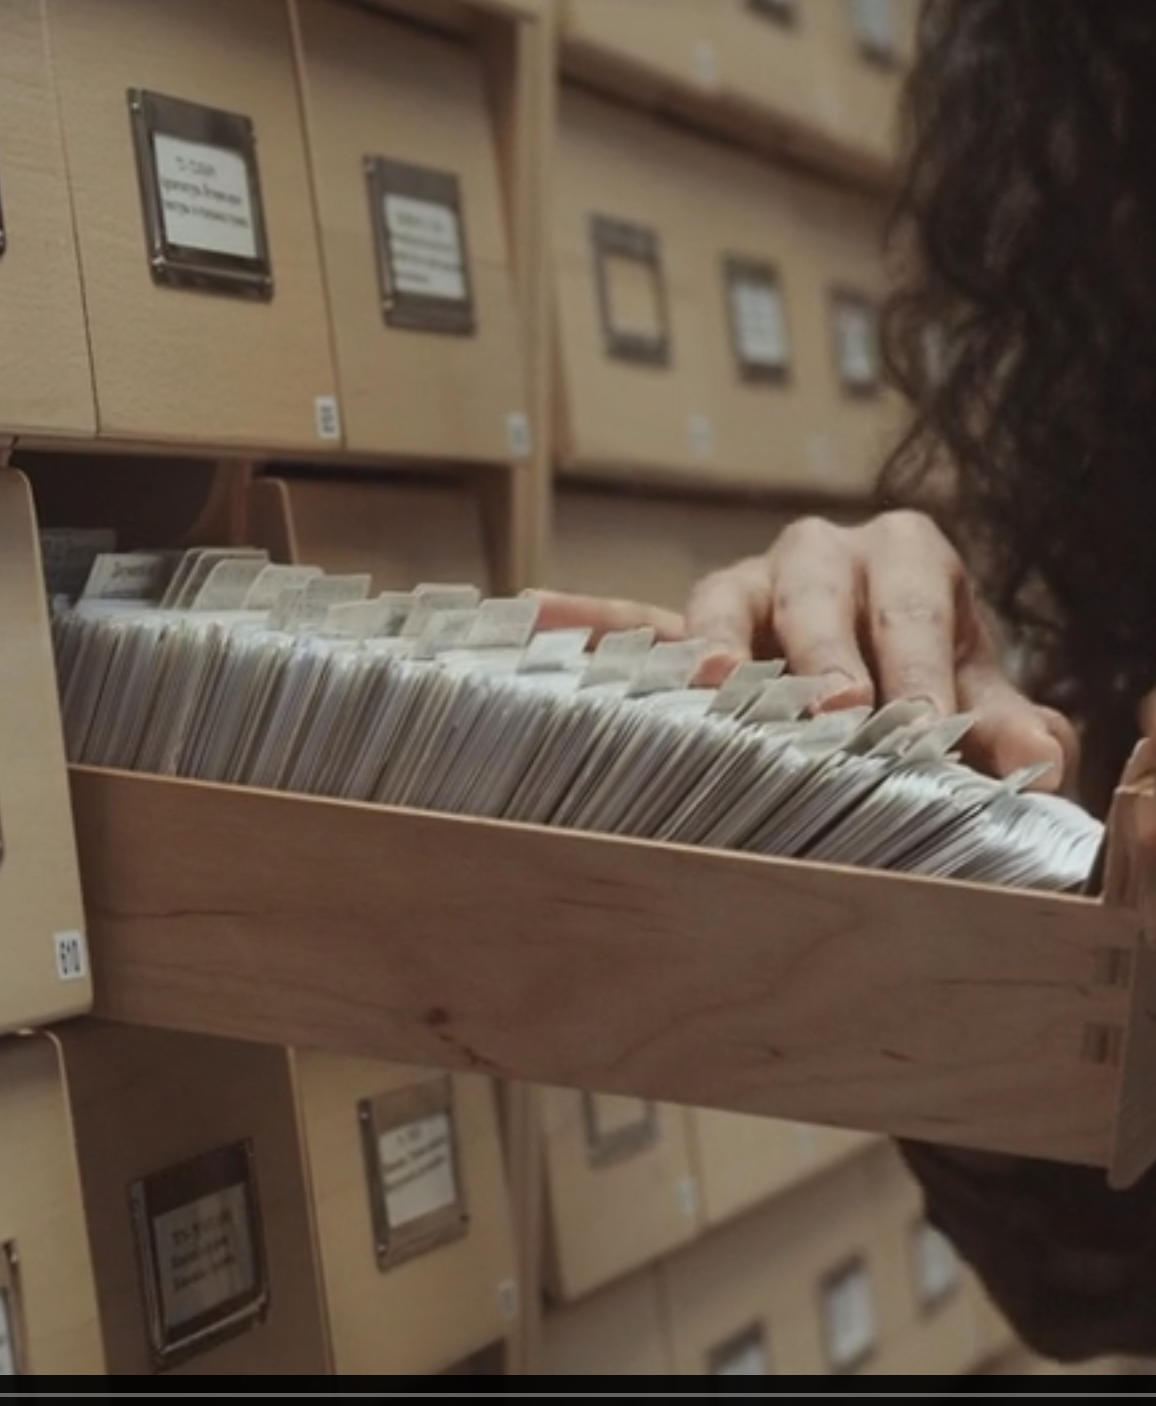
\includegraphics[width=\textwidth]{graphics/Zettelkasten.png}
        \end{column}
        \begin{column}[t]{0.6\textwidth}   
            \vspace{-3.5cm}
            \begin{block}{Der Zettelkasten}
                Eine gute Methode daraus anhaltendes Wissen zu generieren.
                \begin{itemize}
                    \item Atomare Notizen
                    \item Verlinkte Notizen
                    \item Frage/Antwort Zettel
                \end{itemize} 
            \end{block}                     
        \end{column}        
    \end{columns}    
\end{frame}

\begin{frame}{Gute Notizen sind nur die halbe Miete}
    \begin{columns}
        \begin{column}{0.4\textwidth}
            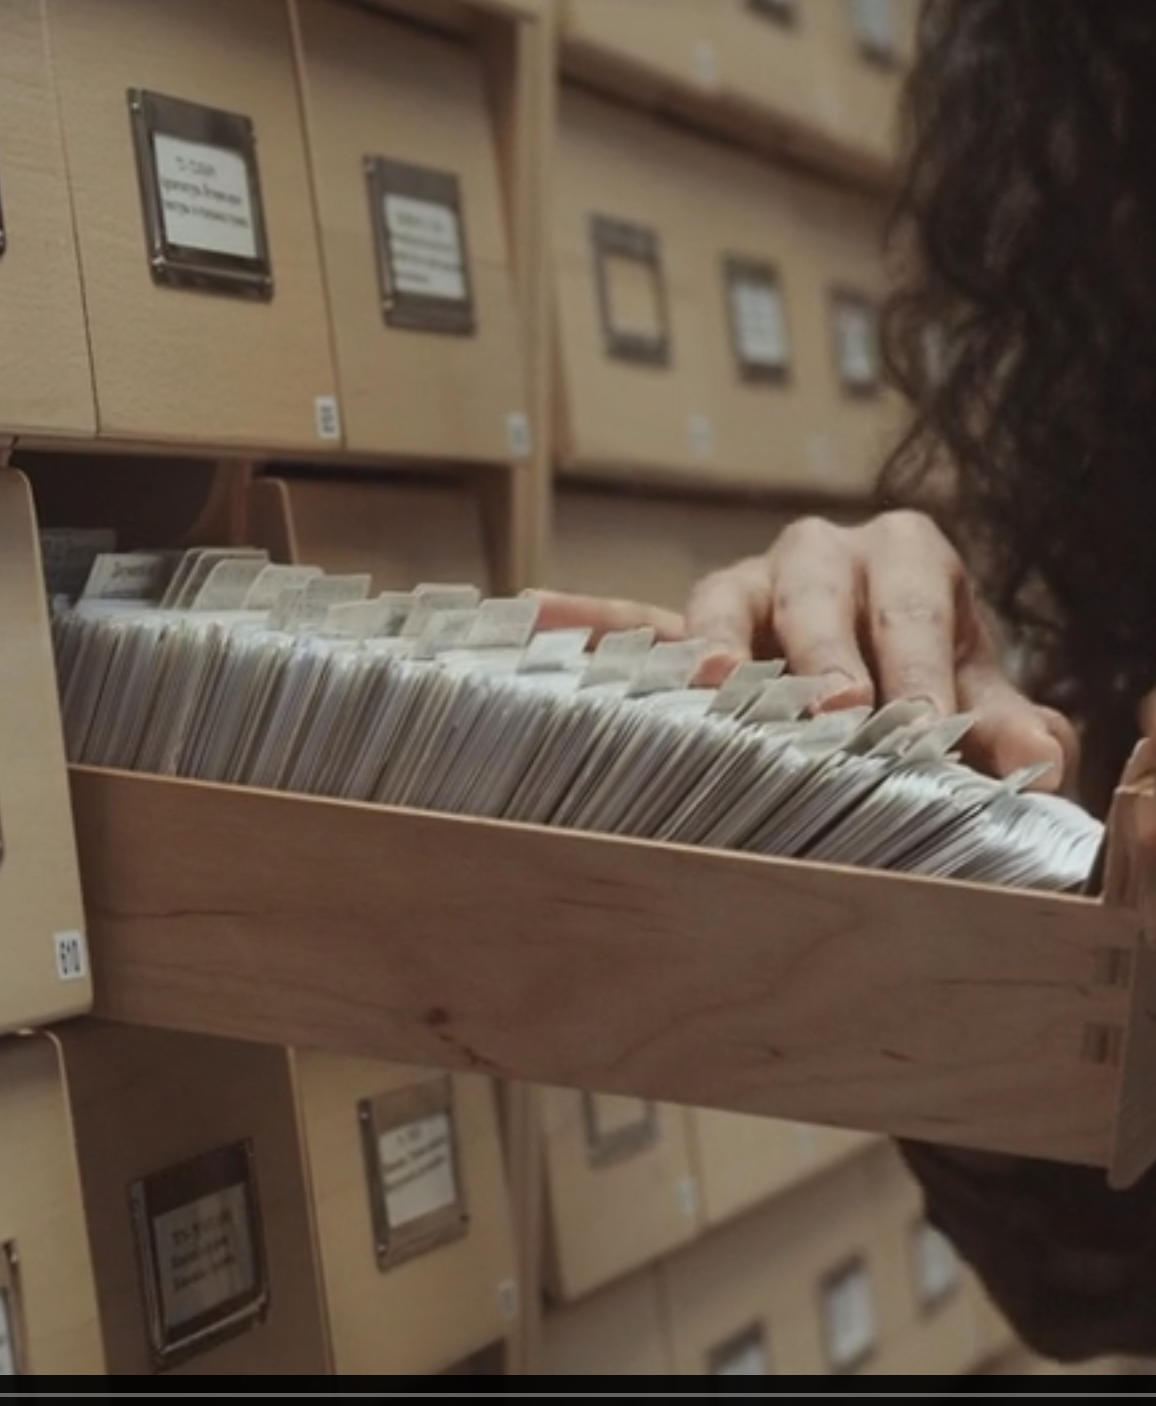
\includegraphics[width=\textwidth]{graphics/Zettelkasten.png}
        \end{column}
        \begin{column}[t]{0.6\textwidth} 
            \vspace{-4cm}
            \begin{figure}[h]
                
\includegraphics[width=\textwidth]{graphics/Logos/anki.png}
            \end{figure}  
            \begin{block}{Karteikarten mit Anki}
                Einfaches Erstellen von Lernkarten
                Clients für PC/Mac und Android/iOS
                
            \end{block}                     
        \end{column}        
    \end{columns}    
\end{frame}

\begin{frame}{Gute Notizen sind nur die halbe Miete}
    \begin{columns}
        \begin{column}{0.4\textwidth}
            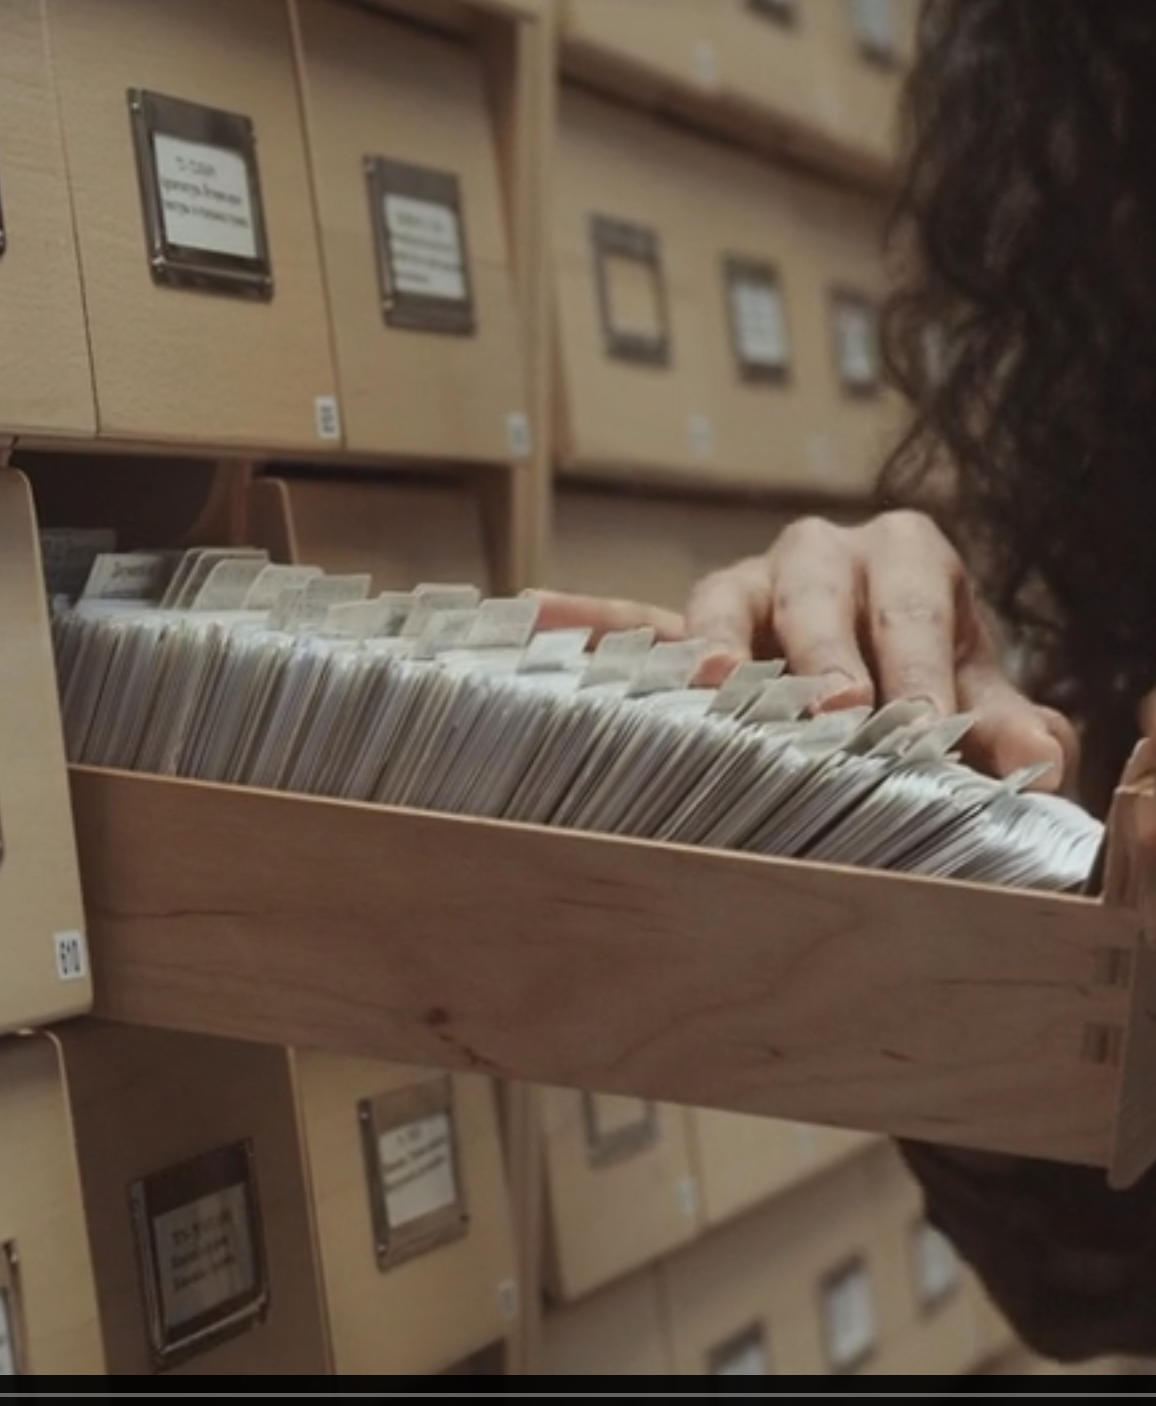
\includegraphics[width=\textwidth]{graphics/Zettelkasten.png}
        \end{column}
        \begin{column}[t]{0.6\textwidth}
            \vspace{-3cm}
            \begin{itemize}[]
                \item Mindmaps
                \begin{itemize}
                    \item Excalidraw
                    \item freeplan.com
                \end{itemize}
                \item Visualisierung
                \begin{itemize}
                    \item \href{https://explaineverything.com/}{Explain Everything}
                    \item \href{https://www.drawio.com/}{Drawio}
                \end{itemize}
            \end{itemize} 


            
        \end{column}        
    \end{columns}    
\end{frame}

\begin{frame}{Kommunikation}
    \begin{columns}[t]
        \begin{column}{0.4\textwidth}
            \vspace{-2em} 
            \begin{figure}
                \begin{flushleft}
                    
\includegraphics[height=0.8\textheight,trim={4cm 0 17cm 0},clip]{graphics/call-2946023_1280.jpg}
                    \caption*{\href{https://pixabay.com/photos/call-afro-megaphone-scream-symbol-2946023/}{fietzfotos on pixabay}}    
                \end{flushleft}                
            \end{figure}            
        \end{column}
        \begin{column}{0.6\textwidth}
            \begin{itemize}
                \item WhatsApp, Telegram
                \item Slack
                \item Matrix        
                \item Discord
                \begin{itemize}
                    \item Kostenlos
                    \item Unterstützt Text, Voice und Video Chats
                    \item Gruppen ermöglichen Organistion der Kommunikation
                \end{itemize}    
            \end{itemize}
        \end{column}
    \end{columns}
\end{frame}

\begin{frame}{Kommunikation}
    \begin{columns}[t]
        \begin{column}{0.4\textwidth}
            \vspace{-2em} 
            \begin{figure}
                \begin{flushleft}
                    
\includegraphics[height=0.8\textheight,trim={4cm 0 17cm 0},clip]{graphics/call-2946023_1280.jpg}
                    \caption*{\href{https://pixabay.com/photos/call-afro-megaphone-scream-symbol-2946023/}{fietzfotos on pixabay}}    
                \end{flushleft}                
            \end{figure}            
        \end{column}
        \begin{column}{0.6\textwidth}
            Communities:
            \begin{itemize}
                \item Reddit 
                \begin{itemize}
                    \item Communities zu methoden, Fächern und Tools mit vielen hilfsbereiten Mitgliedern
                \end{itemize} 
                \item YouTube 
                \item Discord Server
                \begin{itemize}
                    \item Hard zu finden, aber ein guter Interaktionsort für spezifische Themen.
                \end{itemize}        
            \end{itemize}
        \end{column}
    \end{columns}
\end{frame}